\documentclass[12pt]{article}
\usepackage{fullpage,graphicx,psfrag,amsmath,amsfonts,verbatim}
\usepackage[small,bf]{caption}
\usepackage{amsthm}
\usepackage{hyperref}
\usepackage{bbm} % for the indicator function to look good
\usepackage{color}
\usepackage{mathtools}
\usepackage{fancyhdr} % for the header
\usepackage{booktabs} % for regression table display (toprule, midrule, bottomrule)
\usepackage{adjustbox} % for regression table display
\input newcommand.tex
\bibliographystyle{apalike}
% \setlength{\parindent}{0pt} % remove the automatic indentation

\title{L'Hopital's (Selection) Rule: A Bayesian Application to French Hospitals}
\author{Fu Zixuan \\
    Supervised by Thierry Magnac \thanks{Last compiled on \today}}
\date{July 4, 2024}
\begin{document}
\maketitle

\begin{abstract}
    \noindent  Something interesting\\

    % \noindent\textbf{Keywords:} \\

    \bigskip
\end{abstract}

\newpage
\tableofcontents
\newpage

\section{Introduction}

It is almost of human nature to compare, rank and select. And competition, be
it good or bad, emerges in the wake. As invidious as ranking and selection can
be, in many cases it is one of the driving forces behind improvement in
performances. The society itself is constantly constructing league table as
well. It rewards the meritorious and question or even punishes the
unsatisfactory. The measure based on which rank is constructed ranges from
teacher's evaluation to communities' mobility index.

The present article extends the practice to the health sectors. To be more
specific, it studies the labor efficiency across all hospitals in France. By
exploring a comprehensive database (SAE) of French hospitals, I first construct
a measure of labor efficiency. Then based on the estimates, we compare the
public and private hospitals by selecting the top-performing units. I borrow
from the recent developments in Empirical Bayes method to achieve the
comparison.

I found that out of the top 20\% hospitals, there are roughly 9 times

% 658

The article bridges two fields of interests. One is on productivity analysis.
The most popular methods are Data Envelopment Analysis
\cite{charnes1978measuring} and Stochastic Frontier Analysis
\cite{aigner1977formulation,meeusen1977efficiency}. Yet we abstract from both
of them for the convenience of statistical inference. We use the simple method
applied in \cite{croiset2024hospitals} by estimating a conditional input demand
function. To put it simply, we estimate a linear function of how much labor
input is needed to produce a give list of outputs \footnote{We refer the
    audience to xxx for detailed reasons of adopting this approach.}. We only focus
on the employment level of nurses for (reasons) \footnote{} in the
specification.

The second area of interests is the Empirical Bayes Methods. The name
"Empirical Bayes" is self-telling in the sense that Bayes implies a prior
distribution while Empirical means empirically estimate the prior from the
data. Details on how it can be of use in ranking and selection will be
presented in the rest of the section.

In \cite{croiset2024hospitals}, the authors argue that public hospital is less
efficient than private counterpart in the sense that it would need a smaller
size of personnel if it were to use the input demand function of the private
hospital, which is the main result of their counterfactuals.

Having roughly replicated the results after doubling the length of the panel,
the paper differentiates itself by including/adding the standard/classical
panel data methods in input demand function estimation, specifically the
fixed-effect within-group estimation and GMM.

With respect to the latter estimator, we may relax the assumption of strict
exogeneity of the regressors, claiming that current regressors (output) may be
endogeneous/affect current and future errors term.
\begin{equation*}
    y_{it}  = x_{it} \beta + \theta y_{i,t-1}+\theta_i + \varepsilon_{it} \quad  \E\bra{\varepsilon_{it}|x_{i1},\ldots,x_{it-1}} =0
\end{equation*}
Note that the panel used in my estimation has relatively high persistency in the variables. This kind of characteristics was pointed out in \cite{blundell1998initial} as well. It argues that when $T$ is relatively small and the regressors exhibit relatively high auto correlation, the lagged levels of regressors $x_{i,t-2}$ only serve as weak instruments for first differences equation $\Delta \varepsilon_{i,t}$. By imposing a reasonable assumption that $\E{\Delta x_{i,t-1}\varepsilon_{i,t}}$, I instrument the current level with lagged first differences, implementing the so-called system GMM explained in \cite{arellano1995another,blundell1998initial}.

Though the original focus of the panel data estimator is on the $\beta$
parameters. It also provides us with a noisy estimate of the underlying
unobserved heterogeneity term denoted as $\theta_i$. (It's important to note
that this heterogeneity is not necessarily indicative of inefficiency). Now
that we have set the stage for empirical bayes, it is time to bring about the
prior distribution of $\theta_i$, denoted as $G_{\theta}$. If the prior
distribution $G$ is known, having observed an estimate $\hat{\theta}_i$ of
$\theta_i$, we can update our noisy estimate $\hat{\theta}_i$ using or
incorporating our knowledge of $G$.

The usefulness of a prior $G$ is further exemplified/highlighted in the ranking
and selection problem mentioned above, when the object of interests is the
noisy estimate of $\theta_i$. For example, in \cite{gu2023invidious}, we are
given the task of selecting the top 20\% out of the population of $\theta_i$,
that is to say selecting those $i$ whose $alpha_i>G^{-1}(0.8)$, while
controlling for the overall false discovery rate ($\frac{x}{y}$) at 5\%. In
\cite{gu2023invidious}, the authors try to develop an optimal decision rule for
the given task. To put it in the language of optimization, they want to have a
decision rule that optimizes the performance of selection, equivalently,
minimize the loss of selection
\begin{equation*}
    \delta^* = \min_{\delta} \text{Loss} \quad \text{subject to contstraints}
\end{equation*}
where the loss function can take different forms, for example the
expected number of total type 1 and 2 mistakes.

The task at hand falls naturally under the compound decision framework
pioneered by \cite{herbert1956empirical} if we define the loss function in such
a way that takes into account the results of all the individual decisions
$\delta(Y_i)$. For instance, summing all mistakes would be one way to
aggregate/compound individual decisions,

It is obvious that in order to impose the two stated constraints (capacity and
FDR) in formulating the optimization problem, we need to know the prior
distribution $G$. Despite the importance of the $G$, it does not fall from
heaven. Therefore, Empirical Bayes methods come to the rescue, as its name
suggests, we will have to empirically estimating the unknown prior $G$.

Often times "empirically estimating \(G\)" is done with parametric assumption
that \(G\) is normal. Notable use cases are found in teacher evaluation
\cite{chetty2014measuring}, social mobility in communities
\cite{chetty2018impacts} and job discrimination \cite{kline2021reasonable}. By
assuming a Gaussian $G$, they shrink the estimated fixed effect linearly, thus
giving the name "linear shrinkage". However, departure from normality may
render the linear shrinkage rule as unhelpful. Thanks to the foundational work
of \cite{kiefer1956consistency} who has shown that non-parametric estimation is
also feasible and consistent, it is preferable to relax the normality
assumption and estimate the prior $G$ non-parametrically. In terms of
computation method, \cite{koenker2014convex} has formulated the non-parmetric
estimation as a convex optimization problem. Compared to other popular methods
such as EM algorithm \cite{laird1978nonparametric}, recent advancements in
convex optimization computation methods \cite{andersen2010mosek} has made the
novel approach of \cite{koenker2014convex} computationally more attractive.

It is worth mentioning here that though a discrete $G$ with at most x atoms can
be estimated using the REBayes package \cite{koenker2017rebayes}, we are not
free of imposing any assumptions, that is the distribution of estimate
$\hat{\theta}_i|\theta_i,\sigma_i^2.$ To illustrate, in the case of the
estimate of fixed effect, we have

\begin{align*}
    \hat{\theta}_i & =\frac{1}{T}\sum_t (y_{it}-x_{it}\hat{\beta})                         \\
                   & =\frac{1}{T}\sum(\theta_i+\varepsilon_{it}+x_{it}(\beta-\hat{\beta})) \\
                   & \to^d \theta_i+\frac{1}{T}\sum_t \varepsilon_{it}                     \\
\end{align*}

The asymptotic distribution follows from the consistency of $\hat{\beta}$ when
$N \to \infty$, a reasonable assumption in wide panels.

If we may boldly assume that the errors are $i.i.d.$ normally distributed for
each $i$
\begin{equation*}
    \varepsilon_{it} \sim N(0, \sigma_i^2)
\end{equation*}
Then a fixed/small $T$ won't do jeopardize/imperil xxx our argument too much since we do not need to invoke central
limit theorem to have
\begin{equation*}
    \hat{\theta}_i\to^d N(\theta_i,\sigma_i^2/T)
\end{equation*}
However without the normality assumption on the error terms, we have to resort to the
central limit theorem from the claim that $T\to \infty$, which may seem unrealistic for a wide panel ($N>>T$).

The rest of the paper is organized as follows. Section 2 briefly describes the
data and lays out the reduced form estimation of the input demand function,
treating the number of nurses as the dependent variable and a list of 9 output
measures as the regressors. It then applies the classical panel data estimators
to the same specification, distinguishing between whether strict exogeneity is
assumed. In section 3, we introduce the compound decision framework and
specifically/xxx define the selection problem, we then . Section 4 follows with
a comparison of the different selection outcome as a result of imposing varying
constraints and assumptions. We try to draw preliminary conclusion on the
comparative performance of public and private hospitals. Section 5 discusses
potential issues and concludes.

\section{Data and Estimation}
\subsection{Data}
The data we used is called \textit{The Annual Statistics of Health
    Establishments
    (SAE)}\footnote{\href{https://data.drees.solidarites-sante.gouv.fr/explore/dataset/708_bases-statistiques-sae/information/}{La
        Statistique annuelle des établissements (SAE)}}. It is a comprehensive,
mandatory administrative survey and the primary source of data on all health
establishments in France. We primarily exploited the report of healthcare
output (a list of 10 output measure) and labor input (registered and assistant
nurses). The panel covers 9 years from 2013 to 2022, with 2020 missing due to
the pandemic. The number of healthcare units is rather stable. The SAE data
only distinguishes 3 types of units based on legal status. \textit{
    \begin{enumerate}
        \item Ordinary public hospitals
        \item Private for-profit hospitals
        \item Private non-profit hospitals
    \end{enumerate}}
Following \cite{croiset2024hospitals}, we further single out the \textit{public teaching hospitals} because its main objective consists not only of patient treatment, but also teaching and research by and large.

\begin{table}
    \begin{tabular}{rrrrrrr}
        \toprule
          & Year & Teaching & Normal Public & Private For Profit & Private Non Profit & Total \\
        \midrule
        1 & 2013 & 198      & 1312          & 1305               & 1382               & 4197  \\
        2 & 2014 & 201      & 1274          & 1293               & 1349               & 4117  \\
        3 & 2015 & 211      & 1275          & 1297               & 1349               & 4132  \\
        4 & 2016 & 212      & 1266          & 1297               & 1313               & 4088  \\
        5 & 2017 & 211      & 1249          & 1297               & 1306               & 4063  \\
        6 & 2018 & 214      & 1247          & 1296               & 1288               & 4045  \\
        7 & 2019 & 214      & 1236          & 1287               & 1281               & 4018  \\
        8 & 2021 & 219      & 1222          & 1293               & 1264               & 3998  \\
        9 & 2022 & 220      & 1220          & 1296               & 1259               & 3995  \\
        \bottomrule
    \end{tabular}
\end{table}

\textbf{Summarize the output categories}

\begin{adjustbox}{width=1\textwidth}
    \begin{tabular}{rlllll}
        \toprule
          & Output                            & Normal Public & Private Non Profit & Private For Profit & Teaching \\
        \midrule
        1 & STAC inpatient                    & 8.08\%        & 5.66\%             & 16.3\%             & 7.9\%    \\
        2 & STAC oupatient                    & 2.26\%        & 4.02\%             & 22.61\%            & 3.59\%   \\
        3 & Sessions                          & 4.34\%        & 23.31\%            & 27.17\%            & 4.8\%    \\
        4 & Outpatient Consultations          & 58.23\%       & 43.55\%            & 0.8\%              & 69.18\%  \\
        5 & Emergency                         & 21.14\%       & 6.78\%             & 17.3\%             & 12.64\%  \\
        6 & Follow-up care and Long-term care & 1.67\%        & 11.26\%            & 12.16\%            & 1.09\%   \\
        7 & Home hospitalization              & 0.06\%        & 0.76\%             & 0.17\%             & 0.08\%   \\
        8 & Psychiatry stays                  & 4.22\%        & 4.66\%             & 3.49\%             & 0.72\%   \\
        \bottomrule
    \end{tabular}
\end{adjustbox}

\textbf{Summarize the input}: explain the reason why we use nurses instead of medical doctors.

% \begin{adjustbox}{width=1\textwidth}
%     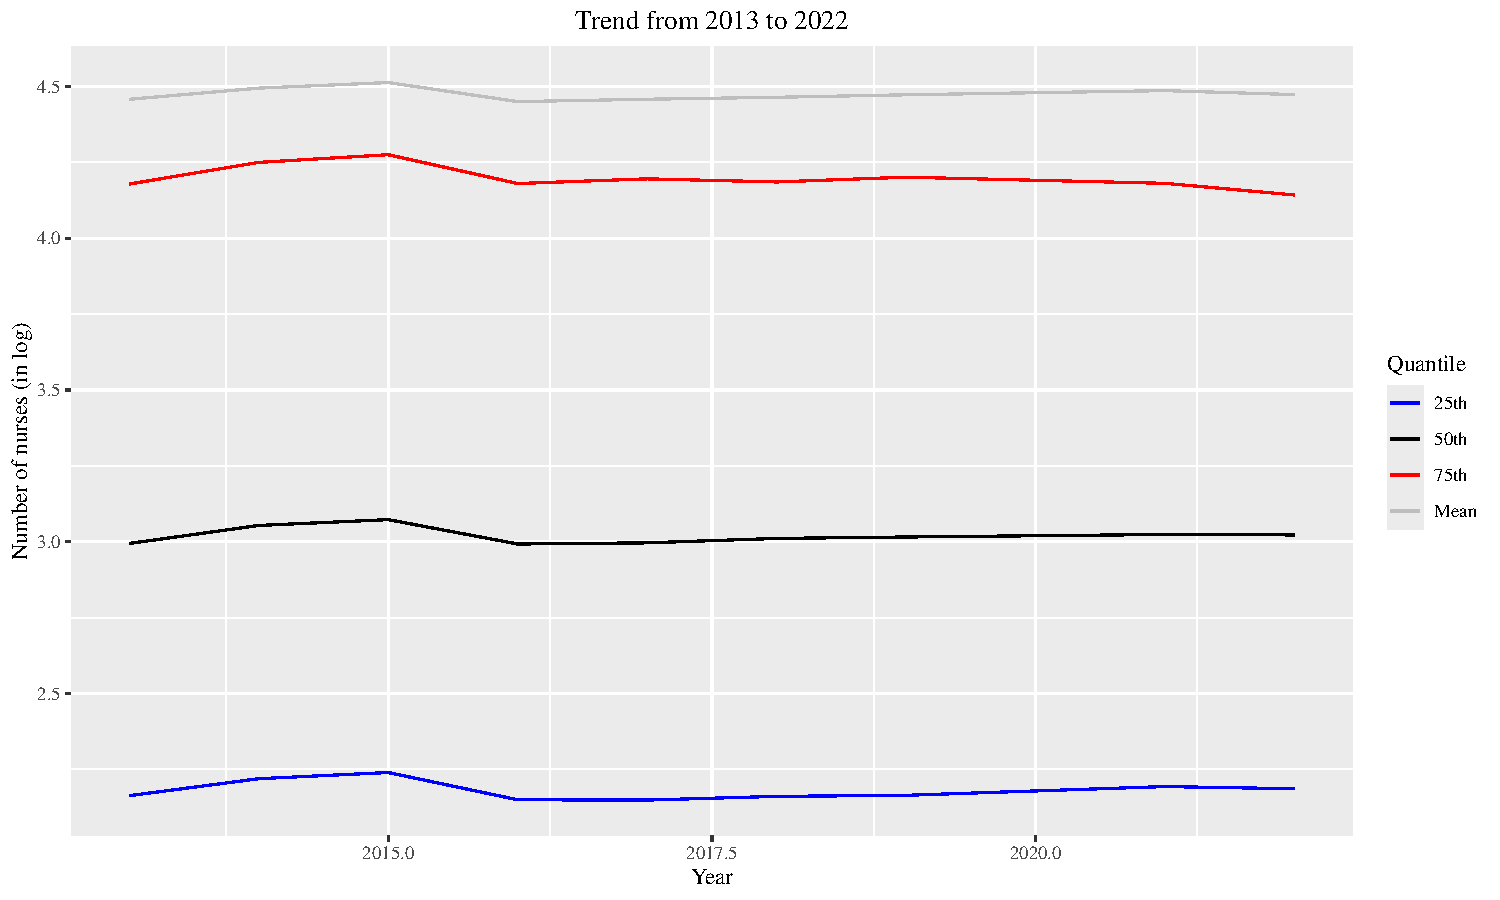
\includegraphics{../../Figures/Descriptive/nurses.pdf}
% \end{adjustbox}

\subsection{Estimation (Pooling)}

\footnote{On a side note, we filtered the panel such that
    \begin{enumerate}
        \item the number of nurses is positive,
        \item at least one of STAC inpatient, STAC outpatient, Sessions is positive,
        \item the number of observations is larger than 6
    \end{enumerate}}

\begin{table}
    
\begingroup
\centering
\begin{tabular}{lcccc}
   \tabularnewline \midrule \midrule
   Dependent Variable: & \multicolumn{4}{c}{Nurses}\\
                           & Pool          & Pool IV       & Dummy          & Dummy IV \\   
   Model:                  & (1)           & (2)           & (3)            & (4)\\  
   \midrule
   \emph{Variables}\\
   Constant                & 1.38$^{***}$  & 1.39$^{***}$  & 1.59$^{***}$   & 1.58$^{***}$\\   
                           & (0.022)       & (0.025)       & (0.025)        & (0.027)\\   
   STAC inpatient          & 0.282$^{***}$ & 0.279$^{***}$ & 0.277$^{***}$  & 0.276$^{***}$\\   
                           & (0.005)       & (0.005)       & (0.004)        & (0.005)\\   
   STAC outpatient         & 0.049$^{***}$ & 0.050$^{***}$ & 0.056$^{***}$  & 0.057$^{***}$\\   
                           & (0.003)       & (0.003)       & (0.003)        & (0.004)\\   
   Medical sessions        & 0.062$^{***}$ & 0.061$^{***}$ & 0.064$^{***}$  & 0.063$^{***}$\\   
                           & (0.002)       & (0.002)       & (0.002)        & (0.002)\\   
   External consultations  & 0.052$^{***}$ & 0.057$^{***}$ & 0.024$^{***}$  & 0.027$^{***}$\\   
                           & (0.001)       & (0.002)       & (0.002)        & (0.002)\\   
   Emergency               & 0.019$^{***}$ & 0.016$^{***}$ & 0.022$^{***}$  & 0.021$^{***}$\\   
                           & (0.001)       & (0.001)       & (0.001)        & (0.001)\\   
   Long-term \& follow-up  & 0.076$^{***}$ & 0.076$^{***}$ & 0.068$^{***}$  & 0.069$^{***}$\\   
                           & (0.002)       & (0.002)       & (0.002)        & (0.002)\\   
   Home care               & 0.018$^{***}$ & 0.016$^{***}$ & 0.027$^{***}$  & 0.026$^{***}$\\   
                           & (0.003)       & (0.003)       & (0.003)        & (0.003)\\   
   Psychiatric care        & 0.075$^{***}$ & 0.073$^{***}$ & 0.064$^{***}$  & 0.063$^{***}$\\   
                           & (0.003)       & (0.003)       & (0.003)        & (0.003)\\   
   Private Forprofit       &               &               & -0.282$^{***}$ & -0.270$^{***}$\\   
                           &               &               & (0.023)        & (0.027)\\   
   Private Nonprofit       &               &               & -0.198$^{***}$ & -0.180$^{***}$\\   
                           &               &               & (0.020)        & (0.021)\\   
   STJR0                   &               &               & 0.713$^{***}$  & 0.707$^{***}$\\   
                           &               &               & (0.020)        & (0.021)\\   
   \midrule
   \emph{Fit statistics}\\
   Observations            & 15,335        & 13,402        & 15,335         & 13,402\\  
   R$^2$                   & 0.820         & 0.821         & 0.837          & 0.838\\  
   \midrule \midrule
   \multicolumn{5}{l}{\emph{Heteroskedasticity-robust standard-errors in parentheses}}\\
   \multicolumn{5}{l}{\emph{Signif. Codes: ***: 0.01, **: 0.05, *: 0.1}}\\
\end{tabular}
\par\endgroup



\end{table}

\begin{table}
    
\begingroup
\centering
\begin{tabular}{lcccc}
   \tabularnewline \midrule \midrule
   Dependent Variable: & \multicolumn{4}{c}{log(ETP\_INF)}\\
                      & Teaching    & Public      & Forprofit   & Nonprofit \\   
   Model:             & (1)         & (2)         & (3)         & (4)\\  
   \midrule
   \emph{Variables}\\
   Constant           & 3.28$^{a}$  & 1.38$^{a}$  & 1.40$^{a}$  & 1.00$^{a}$\\   
                      & (0.328)     & (0.262)     & (0.095)     & (0.149)\\   
   log(SEJHC\_MCO)    & 0.108$^{b}$ & 0.331$^{a}$ & 0.261$^{a}$ & 0.344$^{a}$\\   
                      & (0.042)     & (0.048)     & (0.015)     & (0.034)\\   
   log(SEJHP\_MCO)    & 0.132$^{a}$ & 0.078$^{a}$ & 0.048$^{a}$ & 0.046$^{c}$\\   
                      & (0.032)     & (0.013)     & (0.011)     & (0.027)\\   
   log(SEANCES\_MED)  & 0.060$^{a}$ & 0.051$^{a}$ & 0.075$^{a}$ & 0.094$^{a}$\\   
                      & (0.020)     & (0.007)     & (0.006)     & (0.016)\\   
   log(CONSULT\_EXT)  & 0.017       & 0.025$^{a}$ & -0.003      & 0.001\\   
                      & (0.014)     & (0.008)     & (0.011)     & (0.012)\\   
   log(PASSU)         & 0.049$^{a}$ & -0.009      & 0.033$^{a}$ & 0.025$^{b}$\\   
                      & (0.011)     & (0.008)     & (0.005)     & (0.010)\\   
   log(ENTSSR)        & 0.058$^{a}$ & 0.052$^{a}$ & 0.057$^{a}$ & 0.118$^{a}$\\   
                      & (0.013)     & (0.008)     & (0.008)     & (0.019)\\   
   log(SEJ\_HAD)      & 0.022       & 0.028$^{a}$ & 0.049$^{a}$ & -0.011\\   
                      & (0.027)     & (0.007)     & (0.018)     & (0.022)\\   
   log(SEJ\_PSY)      & 0.026$^{b}$ & 0.070$^{a}$ & 0.084$^{a}$ & 0.045\\   
                      & (0.011)     & (0.010)     & (0.018)     & (0.046)\\   
   \midrule
   \emph{Fit statistics}\\
   Observations       & 1,123       & 5,260       & 4,415       & 2,604\\  
   R$^2$              & 0.779       & 0.860       & 0.742       & 0.754\\  
   \midrule \midrule
   \multicolumn{5}{l}{\emph{Clustered (FI) standard-errors in parentheses}}\\
   \multicolumn{5}{l}{\emph{Signif. Codes: a: 0.01, b: 0.05, c: 0.1}}\\
\end{tabular}
\par\endgroup



\end{table}

A simple counterfactual to perform:
% insert a table where we compare the number of nurses needed in public hospitals if they were to use the input demand function of private hospitals.

\subsection{Estimation (Fixed effect)}
Though \cite{croiset2024hospitals} has mentioned that identification (and
significance level) is mainly attributed to \textit{between-group} variation,
there's still some level of \textit{within-group} variation that guarantee the
estimation of parameters.

The strict exogeneity assumption is not always realistic, especially in the
case of production or factor demand function estimation. Therefore, we resort
to a series of seminal work in panel data estimation
\cite{anderson1982formulation,arellano1991some,arellano1995another,blundell1998initial}.

\begin{table}
    \label{tab:reg_wg_fd_gmm}
    
\begingroup
\centering
\begin{tabular}{lccc}
   \tabularnewline \midrule \midrule
   Dependent Variable:                 & \multicolumn{3}{c}{Nurses}                                   \\
                                       & Within Group               & First Difference & System GMM   \\
   Model:                              & (1)                        & (2)              & (3)          \\
   \midrule
   \emph{Variables}                                                                                   \\
   STAC inpatient                      & $0.10^{***}$               & $0.07^{***}$     & $0.51^{***}$ \\
                                       & $(0.00)$                   & $(0.01)$         & $(0.02)$     \\
   STAC outpatient                     & $0.02^{***}$               & $0.01^{***}$     & $0.06^{***}$ \\
                                       & $(0.00)$                   & $(0.00)$         & $(0.02)$     \\
   Medical sessions                    & $0.02^{***}$               & $0.02^{***}$     & $0.04^{***}$ \\
                                       & $(0.00)$                   & $(0.00)$         & $(0.01)$     \\
   External consultations              & $0.00$                     & $0.00$           & $0.07^{***}$ \\
                                       & $(0.00)$                   & $(0.00)$         & $(0.01)$     \\
   Emergency                           & $0.01^{***}$               & $0.01$           & $-0.07^{**}$ \\
                                       & $(0.00)$                   & $(0.00)$         & $(0.03)$     \\
   Long-term              \& follow-up & $0.01^{***}$               & $0.01^{***}$     & $0.02$       \\
                                       & $(0.00)$                   & $(0.00)$         & $(0.02)$     \\
   Home care                           & $0.01^{***}$               & $0.02^{**}$      & $0.01$       \\
                                       & $(0.00)$                   & $(0.01)$         & $(0.02)$     \\
   Psychiatric care                    & $0.02^{***}$               & $0.01$           & $0.04$       \\
                                       & $(0.00)$                   & $(0.01)$         & $(0.03)$     \\
   \midrule

   \midrule
   \emph{Fit statistics}                                                                              \\
   n                                   & $1690$                     & $1690$           & $1690$       \\
   T                                   & $9$                        & $9$              & $9$          \\
   \midrule \midrule
   \multicolumn{4}{l}{\emph{Signif. Codes: ***: 0.01, **: 0.05, *: 0.1}}                              \\
\end{tabular}
\par\endgroup


\end{table}

It is worth mentioning that the standard first difference GMM where lagged
level $x_{i,t-2}$ is used as instruments for the first difference equation
$\Delta \varepsilon = \Delta y_{i,t}-\Delta x_{i,t} \beta$ does not produce
results of pure noise. This weak instrument issue was pointed out by
\cite{blundell1998initial}.

In the rest of the article, I proceed with the estimation results of system GMM
as in col 3 of Table \ref{tab:reg_wg_fd_gmm}.

\section{Compound Decision: The Selection Problem}
% this is where it finally gets interesting
% from James Stein to Parametric to Non-parametric. Gives an overview of the history of Empirical Bayes Compound Decision

\subsection{Compound Decision}
Leaving the estimation above aside, I will first introduce the idea of compound
decision pioneered by \cite{robbins1956empirical} before entering into the
ranking and selection problem.

Now there are $N$ units, each has an unobserved parameter labelled as
$(\theta_1,\ldots, \theta_n)$. We are given $N$ estimates
$(\hat{\theta}_1,\ldots, \hat{\theta}_n) $ of the underlying heterogeneous
parameters. And each estimate $\hat{\theta}_i$ conditioned on $\theta_i$
follows a distribution $\hat{\theta}_i | \theta_i \sim P_{\theta_i}$. No matter
what the specific task is, I care about the collective performance of my
decision. That being said, I will explicitly define the loss function to
reflect my attention to the so-called collective performance.

First the decision rule is defined as a vector of individual decisions
\begin{equation*}
    \delta(Y) = (\delta_1(\hat{\theta}), \ldots, \delta_n(\hat{\theta}))
\end{equation*}
where each $\delta_i(\cdot)$ is a decision rule for the estimate of $\theta_i$ with the vector $\hat{\theta}$ as input.
The individual loss for a decision is $L(\theta_i, \delta_i(\hat{\theta}_i))$, giving rise to the aggregated \textbf{compound loss}
\begin{equation*}
    L_n(\theta, \delta(\hat{\theta})) = \sum_{i=1}^n L(\theta_i, \delta_i(\hat{\theta})).
\end{equation*}
While the compound risk, defined as the expectation of compound loss can be expressed as
\begin{align*}
    R_n(\theta, \delta(\hat{\theta})) & = \E[L_n(\theta, \delta(\hat{\theta}))]                                                                                                                                    \\
                                      & = \frac{1}{n}\sum_{i=1}^n \E[L(\theta_i, \delta_i(\hat{\theta}))]                                                                                                          \\
                                      & = \frac{1}{n}\sum_{i=1}^n \int \ldots \int L(\theta_i, \delta_i(\hat{\theta}_1, \ldots, \hat{\theta}_n))dP_{\theta_1}(\hat{\theta}_1)\ldots dP_{\theta_n}(\hat{\theta}_n). \\
\end{align*}

Given the objective function which is the compound risk, our goal is to find a
decision rule $\delta(\cdot)$ that minimizes it. This is the optimal compound
decision rule for a given vector $\hat{\theta}$.
\begin{equation*}
    {\delta}^*(\hat{\theta}) =
    \arg\min_{\delta} R_n(\theta, \delta(\hat{\theta}))
\end{equation*}

If $\delta^*(\hat{\theta})$ is separable \footnote{The linear shrinkage class
    belongs to this class as well. See appendix.}, which means that
$\delta^*(\hat{\theta})=\{t(\hat{\theta}_1), \ldots, t(\hat{\theta}_n)\}$, the
compound risk can be written as
\begin{align*}
    R_n(\theta, \delta(\hat{\theta})) f & =  \frac{1}{n}\sum \int\ldots\int L(\theta_i, \delta(\hat{\theta}_1,\dots,\hat{\theta}_n))dP_{\theta_1}(\hat{\theta}_1)\ldots dP_{\theta_n}(\hat{\theta}_n) \\
                                        & = \int_{\theta} \int L(\theta_i, t(\hat{\theta}_i))dP_{\theta_i}(\hat{\theta}_i)dG_n(\theta)                                                                \\
                                        & =\E_{G_n}{\E_\theta\bra{L(\theta_i, \delta_i(\hat{\theta}))}}                                                                                               \\
\end{align*}
where $G_n(\theta)$ is the empirical distribution of $\theta$.\footnote{ $\E_{G_n}\bra{(f(x))} = 1/n \sum_i^n f(x_i)$}

It is worth mentioning that up til now we treat each $\theta_i$ as fixed
unknown parameters \footnote{By abuse of terminology, we called this
    \textit{fixed effect view} while the other assumption \textit{random effect
        view}. Yet the two terms have nothing to do with whether $\theta_i$ is
    correlated with $x_{it}$}. However, if we take a Bayesian view on the vector
$\boldsymbol{\theta}$ by assuming that each $\theta_i$ is an $i.i.d.$ draw from
an underlying common distribution $G$. The Bayesian risk is
\begin{equation*}
    \E_{G}{\E_\theta\bra{L(\theta_i, \delta_i(\hat{\theta}))}}
\end{equation*}
The two views are closely linked via the $G_n$ and $G$.

\begin{quotation}
    Compound Risk is equivalent to the Bayes risk with prior $G_n$.
\end{quotation}

\subsection{Selection Problem}
Our task at hand is to select the top $\alpha\%$ (e.g. 20\%) of the hospitals
in terms of labor use efficiency. If $\theta_i$ represents a measure of
\emph{inefficiency} which is the fixed effect term in the linear input demand
function specified in Section 2. We want to select the top $\theta_i$s that is
below than the $\alpha$ quantile of the population $\theta_i<G_n^{-1}(\alpha)$.
Moreover, we want to subject the selection to another constraint which is the
False Discovery Rate constraint at level $\gamma$, that is
\begin{align*}
    \p\bra{\theta_i>\theta_{\alpha}|\delta_i=1} & =\frac{\p\bra{\theta_i>\theta_{\alpha},\delta_i=1}}{\p\bra{\delta_i=1}}           \\
                                                & = \frac{\E_G\bra{1\set{\theta_i>\theta_{\alpha},\delta_i=1}}}{\E_G\bra{\delta_i}} \\
                                                & \le \gamma                                                                        \\
\end{align*}
Now we are in the position to write down the selection problem subject to the
capacity constraint at $\alpha$ and FDR constraint at $\gamma$ level, with multiplier $\tau_1$ and $\tau_2$ respectively. We denote
$\delta_i=1$ when unit $i$ is selected and $h_i=1\{\theta_i<\theta_\alpha\}=1$ when unit $i$ is truly below
the threshold $\theta_\alpha =G^{-1}(\alpha)$. The compound loss
function is defined as
\begin{equation*}
    L(\delta,\theta)=\sum h_i(1-\delta_i) +\tau_1\pa{\sum (1-h_i)\delta_i -\gamma \delta_i} + \tau_2 \pa{\sum \delta_i -\alpha n}
\end{equation*}
To minimize the compound risk is thus
\begin{align*}
    \min_{\delta} & \E_G\E_{\theta|\hat{\theta}}\bra{L(\delta,\theta)}                                                                                                        \\
                  & =\E_G{\sum \E(h_i)(1-\delta_i) +\tau_1\pa{\sum (1-\E(h_i))\delta_i -\gamma \delta_i} + \tau_2 \pa{\sum \delta_i -\alpha n}}                               \\
                  & =\E_G{\sum v_\alpha(\hat{\theta})(1-\delta_i) +\tau_1\pa{\sum (1-v_\alpha(\hat{\theta}))\delta_i -\gamma \delta_i} + \tau_2 \pa{\sum \delta_i -\alpha n}} \\
\end{align*}
where $v_\alpha(\hat{\theta})=\p(\theta<\theta_\alpha|\hat{\theta})$, which we called \textbf{posterior tail probability}. This is in contrast to the posterior mean widely used to shrink the estimate $\hat{\theta}_i$.
For the moment, it may not immediately obvious how important the prior distribution $G$ is. I will further illustrate it in the next section.
\subsection{Posterior tail probability}
For each $\theta_i$, I observe a sequence of $Y_{it}$ coming from a
longitudinal model
\begin{equation*}
    Y_{it} = \theta_i + \varepsilon_{it} \quad \varepsilon_{it} \sim \caln(0,\sigma_i^2) \quad (\theta_i,\sigma_i^2) \sim G
\end{equation*}
Neither $\theta_i$ nor $\sigma_i^2$ is known to us. But there are two sufficient statistics for $(\theta_i,\sigma_i^2)$.
\begin{align*}
    Y_i=\frac{1}{T_i}\sum_{t=1}^{T_i}Y_{it}           & \quad \text{where}\quad Y_i|\theta_i,\sigma_i^2 \sim \caln(\theta_i,\sigma_i^2/T_i)     \\
    S_i=\frac{1}{T_i-1}\sum_{t=1}^{T_i}(Y_{it}-Y_i)^2 & \quad \text{where} \quad S_i|\sigma_i^2 \sim \Gamma(r_i= (T_i-1)/2,2\sigma_i^2/(T_i-1)) \\
\end{align*}

The tail probability $v_\alpha(y_i,s_i)$ given the two sufficient statistics is
defined as
\begin{align*}
    v_\alpha(Y_i,S_i) & = P( \theta_i > \theta_{\alpha} | Y_i,S_i)                                                                                 \\
                      & = \frac{{\int_{-\infty}^{\theta_{\alpha}} \Gamma(s_i|r_i,\sigma_i^2) f(y_i|\theta_i, \sigma_i^2) dG(\theta_i,\sigma_i^2)}}
    {{\int_{-\infty}^{\infty} \Gamma(s_i|r_i,\sigma_i^2) f(y_i|\theta_i, \sigma_i^2) dG(\theta_i,\sigma_i^2)}}
\end{align*}

\paragraph{Write out the capacity constraint}
\paragraph{Write out the FDR constraint}

If our specification and assumptions on exogeneity are correct, the consistency
of $\hat{\beta}$ is guaranteed by $N$'s asymptotic. However, our estimate of
the fixed effect is
\begin{align*}
    \hat{\theta}_i & =\frac{1}{T}\sum(\theta_i+\varepsilon_{it}+x_{it}(\beta-\hat{\beta}))              \\
                   & \overset{N\to \infty}{\longrightarrow} \theta_i+\frac{1}{T}\sum_t \varepsilon_{it} \\
\end{align*}
When $T$ is relatively small (or even fixed), I am not in a good position to use central limit theorem to claim that $\hat{\theta}_i \overset{d}{\to} \caln(\theta_i,\frac{\sigma_i^2}{T})$. A bold assumption that $\varepsilon_{it} \sim \caln(0,\sigma_i^2)$ will save me from the $T$ issue, which I will impose for the rest of the section (and abstract from whether that  for each $i$ is a testable/reasonable/feasible assumption).

\section{Selection results}

Although \cite{gu2023invidious} has presented the decision rule when
$(\theta_i,\sigma_i^2)$ are unknown. The application assumes that $\sigma_i^2$
is known/observable. In this section, I will compare the selection results
under known variance $\sigma_i^2$ and estimated variance $S_i$.

\paragraph{Known variance, and 4 rules}
\paragraph{Unknown variance, and 4 rules}

\section{Conclusion}

\newpage
\bibliography{ref.bib}

\end{document}
